\chapter{Software Development Process}

\section{Einführung und Motivation}
\subsection{Code and Fix}
Drauf los programmieren, sehen obs funktioniert. Wenn nicht wird es geändert,
so dass es funktioniert. \\

\textbf{Probleme:}
\begin{itemize}
    \item Schlecht strukturierter Code (keine Planung im Voraus)
    \item Nicht systematische Verbesserungen
    \item Schwer im Team umzusetzen, da keine Einteilung existiert
    \item Kein Entwurf oder Dokumentation
    \item Wartbarkeit sehr schwierig (schlechte Doku, keine Struktur)
\end{itemize}

\subsection{Prozessmodell}
Ein Prozessmodell (''Vorgehensmodell'') ist eine abstrakte Repräsentation
des Software Entwicklungsprozesses. Beschreibt den Prozess aus einer bestimmten
Perspektive.\\

\textbf{Richtlinien}
\begin{itemize}
    \item Welche Aktivitäten sollen ausgeführt werden (Wann? In welcher
    Reihenfolge?)
    \item Wer macht was? Rollen und Verantwortlichkeiten
    \item Welche Produkte (Artefakte, Code, Dokumente) sollen bis wann erstellt
    werden
    \item Manchmal welche Techniken und Werkzeuge verwendet werden.
\end{itemize}
\subsubsection{Vorteil von Prozessmodellen}
\begin{itemize}
    \item Klardefinierte Arbeitspakete/Aufgaben $\Rightarrow$ Bessere Verteilung
    auf Team
    \item Fortschritt feststellbar ('' Wo stehe ich in meinem Projekt '')
    \item Verbesserung der Wartbarkeit (Dokumentation)
    \item Geringeres Projektrisiko
    \item Höhere Produktqualität
    \item Explizite Phase der Qualitätssicherung
\end{itemize}
Vorteile hängen jedoch vom konkreten Projekt und den gewählten Prozessen ab.

\section{Wasserfallmodell}
\mbox{}\newline
\begin{figure}[!h]
  \centering
  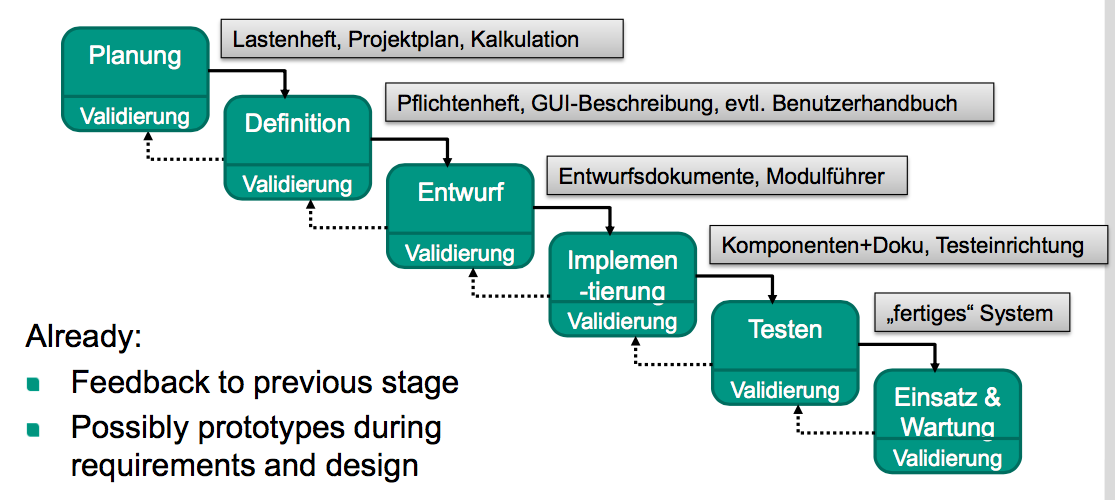
\includegraphics[scale=0.3]{wasserfall}
  \caption{Wasserfall Modell}
\end{figure}

Schwierig umzusetzen, da quasi unmöglich das gesamte System von Anfang an
zu spezifizieren. Bei großen Projekten der Planungshorizont viel zu groß.




\section{Iterative und Inkrementelle Prozesse}

\section{Spiral Model}

\section{Unified Process}
